\documentclass[a4paper]{article}

\def\npart{III Essay}

\def\ntitle{Walking Deeper on Dynamic Graphs}

\def\ndate{\today}

\ifx \nauthor\undefined
  \def\nauthor{Qiangru Kuang}
\else
\fi

\ifx \ntitle\undefined
  \def\ntitle{Template}
\else
\fi

\ifx \nauthoremail\undefined
  \def\nauthoremail{qk206@cam.ac.uk}
\else
\fi

\ifx \ndate\undefined
  \def\ndate{\today}
\else
\fi

\title{\ntitle}
\author{\nauthor}
\date{\ndate}

%\usepackage{microtype}
\usepackage{mathtools}
\usepackage{amsthm}
\usepackage{stmaryrd}%symbols used so far: \mapsfrom
\usepackage{empheq}
\usepackage{amssymb}
\let\mathbbalt\mathbb
\let\pitchforkold\pitchfork
\usepackage{unicode-math}
\let\mathbb\mathbbalt%reset to original \mathbb
\let\pitchfork\pitchforkold

\usepackage{imakeidx}
\makeindex[intoc]

%to address the problem that Latin modern doesn't have unicode support for setminus
%https://tex.stackexchange.com/a/55205/26707
\AtBeginDocument{\renewcommand*{\setminus}{\mathbin{\backslash}}}
\AtBeginDocument{\renewcommand*{\models}{\vDash}}%for \vDash is same size as \vdash but orginal \models is larger
\AtBeginDocument{\let\Re\relax}
\AtBeginDocument{\let\Im\relax}
\AtBeginDocument{\DeclareMathOperator{\Re}{Re}}
\AtBeginDocument{\DeclareMathOperator{\Im}{Im}}
\AtBeginDocument{\let\div\relax}
\AtBeginDocument{\DeclareMathOperator{\div}{div}}

\usepackage{tikz}
\usetikzlibrary{automata,positioning}
\usepackage{pgfplots}
%some preset styles
\pgfplotsset{compat=1.15}
\pgfplotsset{centre/.append style={axis x line=middle, axis y line=middle, xlabel={$x$}, ylabel={$y$}, axis equal}}
\usepackage{tikz-cd}
\usepackage{graphicx}
\usepackage{newunicodechar}

\usepackage{fancyhdr}

\fancypagestyle{mypagestyle}{
    \fancyhf{}
    \lhead{\emph{\nouppercase{\leftmark}}}
    \rhead{}
    \cfoot{\thepage}
}
\pagestyle{mypagestyle}

\usepackage{titlesec}
\newcommand{\sectionbreak}{\clearpage} % clear page after each section
\usepackage[perpage]{footmisc}
\usepackage{blindtext}

%\reallywidehat
%https://tex.stackexchange.com/a/101136/26707
\usepackage{scalerel,stackengine}
\stackMath
\newcommand\reallywidehat[1]{%
\savestack{\tmpbox}{\stretchto{%
  \scaleto{%
    \scalerel*[\widthof{\ensuremath{#1}}]{\kern-.6pt\bigwedge\kern-.6pt}%
    {\rule[-\textheight/2]{1ex}{\textheight}}%WIDTH-LIMITED BIG WEDGE
  }{\textheight}% 
}{0.5ex}}%
\stackon[1pt]{#1}{\tmpbox}%
}

%\usepackage{braket}
\usepackage{thmtools}%restate theorem
\usepackage{hyperref}

% https://en.wikibooks.org/wiki/LaTeX/Hyperlinks
\hypersetup{
    %bookmarks=true,
    unicode=true,
    pdftitle={\ntitle},
    pdfauthor={\nauthor},
    pdfsubject={Mathematics},
    pdfcreator={\nauthor},
    pdfproducer={\nauthor},
    pdfkeywords={math maths \ntitle},
    colorlinks=true,
    linkcolor={red!50!black},
    citecolor={blue!50!black},
    urlcolor={blue!80!black}
}

\usepackage{cleveref}



% TODO: mdframed often gives bad breaks that cause empty lines. Would like to switch to tcolorbox.
% The current workaround is to set innerbottommargin=0pt.

%\usepackage[theorems]{tcolorbox}





\usepackage[framemethod=tikz]{mdframed}
\mdfdefinestyle{leftbar}{
  %nobreak=true, %dirty hack
  linewidth=1.5pt,
  linecolor=gray,
  hidealllines=true,
  leftline=true,
  leftmargin=0pt,
  innerleftmargin=5pt,
  innerrightmargin=10pt,
  innertopmargin=-5pt,
  % innerbottommargin=5pt, % original
  innerbottommargin=0pt, % temporary hack 
}
%\newmdtheoremenv[style=leftbar]{theorem}{Theorem}[section]
%\newmdtheoremenv[style=leftbar]{proposition}[theorem]{proposition}
%\newmdtheoremenv[style=leftbar]{lemma}[theorem]{Lemma}
%\newmdtheoremenv[style=leftbar]{corollary}[theorem]{corollary}

\newtheorem{theorem}{Theorem}[section]
\newtheorem{proposition}[theorem]{Proposition}
\newtheorem{lemma}[theorem]{Lemma}
\newtheorem{corollary}[theorem]{Corollary}
\newtheorem{axiom}[theorem]{Axiom}
\newtheorem*{axiom*}{Axiom}

\surroundwithmdframed[style=leftbar]{theorem}
\surroundwithmdframed[style=leftbar]{proposition}
\surroundwithmdframed[style=leftbar]{lemma}
\surroundwithmdframed[style=leftbar]{corollary}
\surroundwithmdframed[style=leftbar]{axiom}
\surroundwithmdframed[style=leftbar]{axiom*}

\theoremstyle{definition}

\newtheorem*{definition}{Definition}
\surroundwithmdframed[style=leftbar]{definition}

\newtheorem*{slogan}{Slogan}
\newtheorem*{eg}{Example}
\newtheorem*{ex}{Exercise}
\newtheorem*{remark}{Remark}
\newtheorem*{notation}{Notation}
\newtheorem*{convention}{Convention}
\newtheorem*{assumption}{Assumption}
\newtheorem*{question}{Question}
\newtheorem*{answer}{Answer}
\newtheorem*{note}{Note}
\newtheorem*{application}{Application}

%operator macros

%basic
\DeclareMathOperator{\lcm}{lcm}

%matrix
\DeclareMathOperator{\tr}{tr}
\DeclareMathOperator{\Tr}{Tr}
\DeclareMathOperator{\adj}{adj}

%algebra
\DeclareMathOperator{\Hom}{Hom}
\DeclareMathOperator{\End}{End}
\DeclareMathOperator{\id}{id}
\DeclareMathOperator{\im}{im}
\DeclareMathOperator{\coker}{coker}
\DeclarePairedDelimiter{\generation}{\langle}{\rangle}

%groups
\DeclareMathOperator{\sym}{Sym}
\DeclareMathOperator{\sgn}{sgn}
\DeclareMathOperator{\inn}{Inn}
\DeclareMathOperator{\aut}{Aut}
\DeclareMathOperator{\GL}{GL}
\DeclareMathOperator{\SL}{SL}
\DeclareMathOperator{\PGL}{PGL}
\DeclareMathOperator{\PSL}{PSL}
\DeclareMathOperator{\SU}{SU}
\DeclareMathOperator{\UU}{U}
\DeclareMathOperator{\SO}{SO}
\DeclareMathOperator{\OO}{O}
\DeclareMathOperator{\PSU}{PSU}
\DeclareMathOperator{\Sp}{Sp}


%hyperbolic
\DeclareMathOperator{\sech}{sech}

%field, galois heory
\DeclareMathOperator{\ch}{ch}
\DeclareMathOperator{\gal}{Gal}
\DeclareMathOperator{\emb}{Emb}



%ceiling and floor
%https://tex.stackexchange.com/a/118217/26707
\DeclarePairedDelimiter\ceil{\lceil}{\rceil}
\DeclarePairedDelimiter\floor{\lfloor}{\rfloor}


\DeclarePairedDelimiter{\innerproduct}{\langle}{\rangle}

%\DeclarePairedDelimiterX{\norm}[1]{\lVert}{\rVert}{#1}
\DeclarePairedDelimiter{\norm}{\lVert}{\rVert}



%Dirac notation
%TODO: rewrite for variable number of arguments
\DeclarePairedDelimiterX{\braket}[2]{\langle}{\rangle}{#1 \delimsize\vert #2}
\DeclarePairedDelimiterX{\braketthree}[3]{\langle}{\rangle}{#1 \delimsize\vert #2 \delimsize\vert #3}

\DeclarePairedDelimiter{\bra}{\langle}{\rvert}
\DeclarePairedDelimiter{\ket}{\lvert}{\rangle}




%macros

%general

%divide, not divide
\newcommand*{\divides}{\mid}
\newcommand*{\ndivides}{\nmid}
%vector, i.e. mathbf
%https://tex.stackexchange.com/a/45746/26707
\newcommand*{\V}[1]{{\ensuremath{\symbf{#1}}}}
%closure
\newcommand*{\cl}[1]{\overline{#1}}
%conjugate
\newcommand*{\conj}[1]{\overline{#1}}
%set complement
\newcommand*{\stcomp}[1]{\overline{#1}}
\newcommand*{\compose}{\circ}
\newcommand*{\nto}{\nrightarrow}
\newcommand*{\p}{\partial}
%embed
\newcommand*{\embed}{\hookrightarrow}
%surjection
\newcommand*{\surj}{\twoheadrightarrow}
%power set
\newcommand*{\powerset}{\mathcal{P}}

%matrix
\newcommand*{\matrixring}{\mathcal{M}}

%groups
\newcommand*{\normal}{\trianglelefteq}
%rings
\newcommand*{\ideal}{\trianglelefteq}

%fields
\renewcommand*{\C}{{\mathbb{C}}}
\newcommand*{\R}{{\mathbb{R}}}
\newcommand*{\Q}{{\mathbb{Q}}}
\newcommand*{\Z}{{\mathbb{Z}}}
\newcommand*{\N}{{\mathbb{N}}}
\newcommand*{\F}{{\mathbb{F}}}
%not really but I think this belongs here
\newcommand*{\A}{{\mathbb{A}}}

%asymptotic
\newcommand*{\bigO}{O}
\newcommand*{\smallo}{o}

%probability
\newcommand*{\prob}{\mathbb{P}}
\newcommand*{\E}{\mathbb{E}}

%vector calculus
\newcommand*{\gradient}{\V \nabla}
\newcommand*{\divergence}{\gradient \cdot}
\newcommand*{\curl}{\gradient \cdot}

%logic
\newcommand*{\yields}{\vdash}
\newcommand*{\nyields}{\nvdash}

%differential geometry
\renewcommand*{\H}{\mathbb{H}}
\newcommand*{\transversal}{\pitchfork}
\renewcommand{\d}{\mathrm{d}} % exterior derivative

%number theory
\newcommand*{\legendre}[2]{\genfrac{(}{)}{}{}{#1}{#2}}%Legendre symbol

%algebraic geometry
\DeclareMathOperator{\Spec}{Spec}
\DeclareMathOperator{\Proj}{Proj}

\let\SO\undefined
\usepackage{tkz-graph}
\usepackage{thm-restate}
\usepackage{algpseudocode}
\usepackage{algorithm}
\newcommand{\shadow}{\partial}
\renewcommand{\P}{\mathbb P}
\renewcommand{\E}{\mathbb E}
\newcommand{\D}{\mathcal D}
\renewcommand{\G}{\mathcal G}
\renewcommand{\V}{\mathcal V}
\newcommand{\rar}{\overrightarrow r}
\newcommand{\lar}{\overleftarrow r}
\renewcommand{\algorithmicrequire}{\textbf{Input:}}
\renewcommand{\algorithmicensure}{\textbf{Output:}}
\algnewcommand{\LineComment}[1]{\State \(\triangleright\) #1}
\begin{document}

\begin{titlepage}
  \begin{center}
%    \includegraphics[width=0.6\textwidth]{logo.jpg}\par
    \vspace{2cm}
    {\scshape\huge University of \par
      \Huge Cambridge \par}
    \vspace{1cm}
    {\scshape\huge Mathematics Tripos \par}
    \vspace{2cm}
    {\huge Part \npart \par}
    \vspace{0.6cm}
    {\Huge \bfseries \ntitle \par}
    \vspace{1.2cm}
    {\Large\ndate \par}
    \vspace{2cm}
    
    {\large \emph{Written by } \par}
    \vspace{0.2cm}
    {\Large \scshape Joshua Snyder}
 \end{center}
\end{titlepage}

\tableofcontents

\section{Introduction}
The motivation of this essay and the methods it presents comes from the desire to understand networks of people and the relationships between them.
From a mathematical perspective, the natural way to go about studying social networks is to let nodes of a graph G represent the people and edges their relationships. From this, we can induce some understanding of the neighbourhoods that a network consists of. This task of understanding the communities that exist in a social network is a complex one; even with a relatively small number of people it is not a task for which humans perform very well and the task rapidly becomes difficult as the size of the network increases.\\
Network embeddings are a useful way to characterise the complex structures that
can exist in these graphs. The idea behind them is to represent each member of a
network with a point in space, where the distance according to some metric
(often simply Euclidean) between any two points corresponds to the similarity of
the members in the network. These points in space are called vertex
representations. The difficulty with this approach is defining a suitable
similarity function $f(p1,p2)$ that gives a good understanding of the network
structure. This ambiguity of similarity has led to a diverse range of algorithms for calculating network embeddings.
\begin{figure}[h!]
  \centering
  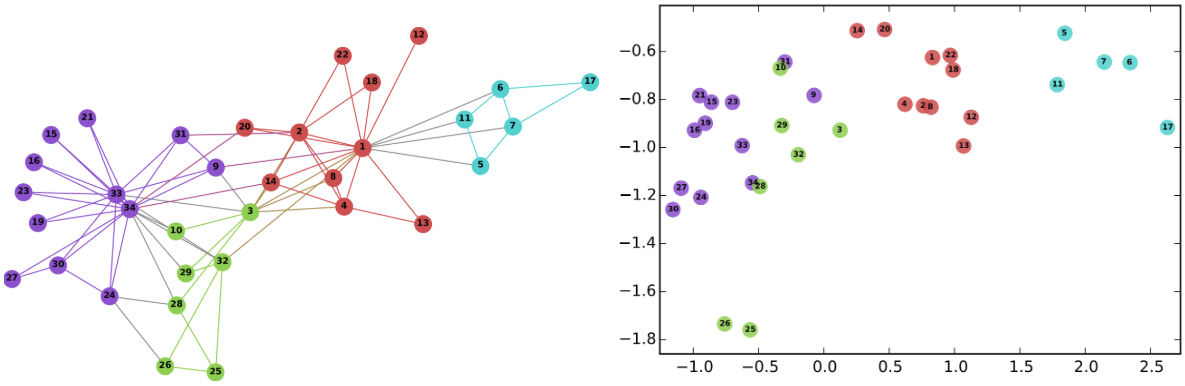
\includegraphics[width = 1\textwidth]{src/DeepWalkOnKarateGraph.png}

  \caption{Two dimensional network embeddings calculated using
    DeepWalk on Zachary's Karate network\cite{zachary1977}. There is a strong
    correspondence between community structure in the original graph and
    in the embedding space. Vertex colours are representing a modularity-based
    clustering of the input graph. In practive, network embeddings have dimensions
    in the tens to low-hundreds and t-SNE is often used to visualise these embeddings in 2D
    space.\cite{maaten2008}}
\end{figure}\\
The problem of analysing social structures is made more difficult still by the
fact that such networks often change over time. As new connections are formed
and others die away, the network moves and over a long time period, it can
change significantly. Calculating the vertex representations for a large social
graph, where the size of the network is often in the millions or billions, takes
a lot of time. It is therefore computationally infeasible to recalculate these
representations at every time step and so a more intelligent approach to this
problem is required.\\
This essay looks at DeepWalk and how it can be modified for dealing with dynamic
graphs. DeepWalk is an algorithm that calculates vertex representations for
large social graphs by using techniques adapted from natural language processing. When proposed in 2014, the algorithm was a first of its kind and has since sparked a large amount of future research, with new algorithms improving upon it using similar methods. The core idea behind DeepWalk is to model random walks on a graph similar to sentences in a large corpus of text, this idea is explored further throughout the essay.


\subsection{Summary}
The section on DeepWalk explores the fundamental connection between DeepWalk and
matrix factorisation as presented in the paper by Qiu et al.\cite{qiu2018}. In
this section, we demonstrate the conditions under which DeepWalk is factorising
an appropriate matrix that stores some measure of similarity between
nodes in the graph. In the section ``Why DeepWalk sucks'' we look at some of the
criticism that followed the original DeepWalk paper and how these criticisms
were addressed by future authors, the section is indicative of the shortcomings
of DeepWalk but is by no means exhaustive.\\
After this, the section ``Dynamic DeepWalking'' focusses on applying a variant of the DeepWalk algorithm, proposed
by Sajjad et al. \cite{sajjad2019}, for dynamic graphs. This is especially
important in the context of social graphs, which usually contain temporal information
about user interactions. Learning social
representations for dynamic graphs can allow for a better understanding of how
communities move and change over time.\\
Finally, to exhibit Dynamic DeepWalking in practice, the final section of this
essay applies the Unbiased Update algorithm introduced by Sajjad et
al.\cite{sajjad2019} to data from users on the social network Gab to look at how
user interaction on the network varies with time. 

\subsection{Preliminary Notation}
I have endeavoured to use similar notation to the original DeepWalk paper\cite{deepwalk} to ease
cross-referencing. However given that a number of other papers are touched upon
throughout the essay, there are some pieces of notation that have been changed.
If reading through the essay systematically, the reader should not find
difficulty following the notation.

\begin{definition}[(Partially Labelled) Network Graph]
  Let $G = (V, E)$ be an undirected graph (representing a network). $V$ represents the
  members of the network, commonly referred to as the \textit{nodes} or \textit{vertices} and $E \subset V
  \times V$ represents their connections, usually referred to as
  \textit{edges}.\\
  The nodes and edges have labels and $G_L = (V, E, X, Y)$ represents the
  partially labelled network. $X \in \R^{|V| \times S}$ where $S$ is the size of
  the feature space for each attribute vector and $Y \in \R^{|V|
    \times|\mathcal{Y}|}$, where $\mathcal{Y}$ is the set of labels.
\end{definition}
*** Note partially labelled graphs have not been touched upon, what are the
labels being used for? Are they being used pre or post embedding? ***
Our goal is to learn embeddings $W \in \R^{|V| \times d}$ where $d$ is a small number
of latent dimensions ($d \ll |V|$) such that each of the rows in $W$
corresponds to a $d$ dimensional embedding of a node in $V$.
\section{DeepWalk}
This section gives an outline of the social representation learning algorithm
DeepWalk, first introduced in the seminal paper DeepWalk: Online Learning of
Social Representations by B. Perozzi et. al. \cite{deepwalk}. The method proposed in
this paper not only demonstrated performance improvements from previous methodologies but
also motivated an entirely different approach. At the time of the paper being
written, significant advancements were being made in natural language processing (NLP)
and the idea of word embeddings was becoming popular through an embedding
algorithm known as Word2Vec \cite{mikolov2013efficient,mikolov2013distributed}.
DeepWalk implements this algorithm but replaces the idea of the context of a word in
a sentence with the context of a node in a random walk on a graph. This is the
crucial concept of DeepWalk from which the remaining details of the algorithm naturally follow.\\
The original paper on DeepWalk is lacking in a mathematical foundation and so in
this section we will model the algorithm mathematically. It is suggested that the reader
is familiar with the concepts outlined in the paper by Perozzi et. al. prior to
reading this (more) mathematical exposition.
\begin{algorithm}
  \caption{DeepWalk}
  \begin{algorithmic}[1]
    \Require{network $G(V, E)$}
    \Statex window size $k$
    \Statex embedding size $d$
    \Statex walks per vertex $\gamma$
    \Statex walk length $l$
    \Ensure{matrix of vertex representations $W \in \R^{|V| \times d}$}
    \State Initialization: Sample $W$ from $\mathcal{U}^{|V| \times d}$
    \For{$i = 0$ to $\gamma$}
    \State $\mathcal{O} = \text{Shuffle}(V)$
    \For{\textbf{each} $v \in \mathcal{O}$}
    \State $\mathcal{W}_v =$ RandomWalk$(G, v, l)$
    \State Skipgram$(W, \mathcal{W}_v, k)$
    \EndFor
    \EndFor
  \end{algorithmic}
\end{algorithm}
\subsection{Introduction to DeepWalk}
To understand DeepWalk mathematically, we first need to understand what the SkipGram
model is doing, since this is the model underpinning DeepWalk. SkipGram was
prposed by Mikolev et al.\cite{mikolov2013efficient} as an efficient way to
learn word embeddings. The idea behind SkipGram is to learn embeddings which are good at
predicting nearby words in sentences. For a sentence $w_1, ... , w_N$, the
nearby words from $w_i$, known as context words, are defined as the set of words
within distance $k$, $\{w_{i-k}, w_{i-k+1}, \dots , w_{i+k}\} \setdiff w_i$, where $k$ is the size of the window. SkipGram
minimises the following objective function
\[\mathcal{L} = - \sum_{c \in C(w)} \log{\P(c | w)}\]
where $\P(c | w)$ is modelled by a softmax function
\[\P(u|v) = \frac{\exp{(\vec{w} \cdot \vec{c}})}{\sum_{c \in \mathcal{F}}\exp{(\vec{w} \cdot
    \vec{c}})}\]
where $\mathcal{F}$ is the vocabulary and $\vec{w}$ represents the
embedding of the word $w$ and $\vec{c}$ the distributed representation of $c$ when it serves as a
context word.\\
*** Can I be clearer about what this distributed representation is? ***\\
Perrozi et al. took this model from NLP and applied it to graphs by observing
that nodes in the graph can be thought of as words in an antificial language.
Firstly, to find the context for each node, DeepWalk generates random walks
which are analagous to sentences in a language. The context nodes are the set of
nodes within a window of size $k$, from which input-context pairs $(v, c)$ are
constructed and added to a corpus $\D$, which is a multi-set. After these context nodes have been
found the same optimization function as in SkipGram is used to learn embeddings which maximise
the chance of predicting context nodes.\\
Algorithm 1 shows how DeepWalk is applied. $\gamma$ represents the number of
random walks that are started from each node and at the start of each pass the
nodes are shuffled so that they are traversed in a random order.\footnote{This
  helps to prevent the algorithm from staying in a local minima when stochastic
  gradient descent is applied since on each iteration, as the vertices
  are shuffled, the shape of the loss surface changes.} For each node
$v \in V$ a random walk $\mathcal{W}_v$ of length $l$ is generated and used to
update the network embeddings using the SkipGram algorithm applied to the random
walk.\\
From the perspective of machine learning, SkipGram trains a neural network to do
a ``fake'' task. It trains on this task, and then the corresponding weights
learned are used as embeddings. The task is as follows:\\
Given an input vertex $v$ somewhere in a random walk $\mathcal{W}$. Pick a
nearby vertex at random. The task of the neural network is to
predict the probability that each vertex in $V$ will be this randomly chosen
vertex. Therefore, verticies far away on the graph that correspond to unfamiliar
nodes are unlikely to co-occur on the same random walk and will be assigned a
low probability. Conversely, nearby and well connected vertices are likely to
co-occur on a random walk with input $v$ and thus will be assigned higher
probabilities. This allows us to train a network with weights that represent the
connectedness between nodes on the graph. The neural network is trained by
feeding it pairs of nodes $(v, c)$ where $v$ represents the input node and $c$
is a context node, which lies within distance $k$ of the vertex $v$.\\ 

To formalise this, each of the nodes $v \in V$ are represented by a one-hot
encoding vector $e_v \in \mathbb{R}^{|V|}$ allowing us to feed $e_v$ into the
neural network. When $e_v$ is fed into the network, a single linear hidden layer with
$d$ neurons is used, where $d$ is the desired dimension of the latent
representations, which is then passed to a softmax classifier for output. The
output of the network is a vector $o \in \mathbb{R}^{|V|}$ containing the estimated
probabilities that a randomly selected nearby word is that vocabulary word.

The idea behind having a linear hidden layer, which does not use an activation
function, is to use the resulting weight matrix $W \in \mathbb{R}^{|V| \times
  d}$ as the embedding vectors for the nodes in the graph. This is intuitive as
the hidden layer acts as a bottleneck that tries to represent as much
information as possible to distinguish the nodes, but is only allowed $d$
neurons to do so. Since $d \ll |V|$ there is a low risk of overfitting.

*** Create here an image resembling the one found in the blog post on SkipGram
but for graphs and with $d$ dimensions ***\\

% This creates the neural network diagram for the SkipGram neural network

\tikzset{%
  every neuron/.style={
    circle,
    draw,
    minimum size=0.6cm
  },
  neuron missing/.style={
    draw=none, 
    scale=3,
    text height=0.2cm,
    execute at begin node=\color{black}$\vdots$
  },
}

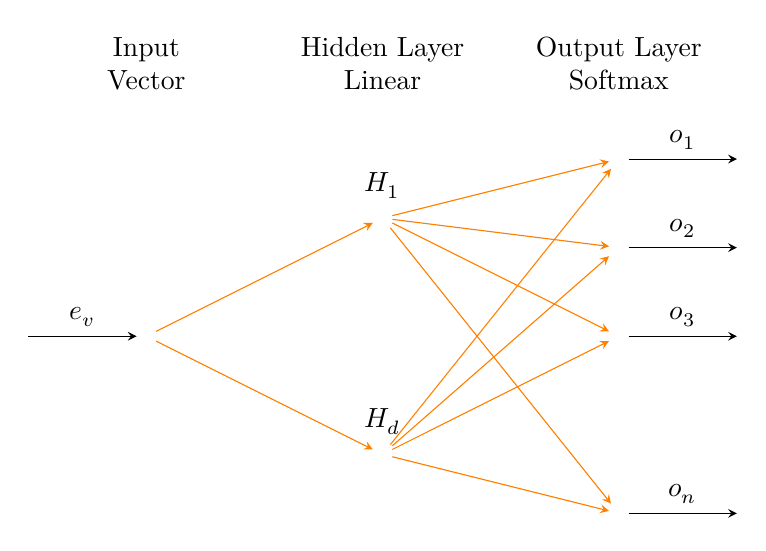
\begin{tikzpicture}[x=1.5cm, y=1.5cm, >=stealth]

\foreach \m/\l [count=\y] in {1}
  \node [every neuron/.try, neuron \m/.try] (input-\m) at (0,0) {};

\foreach \m [count=\y] in {1, missing,2}
  \node [every neuron/.try, neuron \m/.try ] (hidden-\m) at (2,2 - \y) {};

\foreach \m [count=\y] in {1,2,3,missing,4}
  \node [every neuron/.try, neuron \m/.try ] (output-\m) at (4,2.25-\y*0.75) {};

\foreach \l [count=\i] in {1}
  \draw [<-] (input-\i) -- ++(-1,0)
    node [above, midway] {$e_v$};

\foreach \l [count=\i] in {1,d}
  \node [above] at (hidden-\i.north) {$H_\l$};

\foreach \l [count=\i] in {1,2,3,n}
  \draw [->] (output-\i) -- ++(1,0)
    node [above, midway] {$o_{\l}$};

\foreach \i in {1}
  \foreach \j in {1,...,2}
    \draw[orange] [->] (input-\i) -- (hidden-\j);

\foreach \i in {1,...,2}
  \foreach \j in {1,2,3,...,4}
    \draw[orange] [->] (hidden-\i) -- (output-\j);

\node [align=center, above] at (0,2) {Input\\Vector};
\node [align=center, above] at (2,2) {Hidden Layer\\Linear};
\node [align=center, above] at (4,2) {Output Layer\\Softmax};


\end{tikzpicture}\\
The algorithm used in DeepWalk varies slightly from the SkipGram algorithm
discussed. Calculating the normalization factor in the Softmax layer requires a
computational complexity of $O(|V|)$, in the original DeepWalk paper this is
reduced by using Hierarchical Softmax to approximate the softmax probabilities,
requiring a complexity of only $O(log|V|)$. In particular, a Huffman coding is
used to reduce the access time of frequent elements in the tree, as suggested by
Mikolov et al. in the original Word2Vec
papers.\cite{mikolov2013distributed,mikolov2013efficient}

In later adaptations of DeepWalk, SkipGram with Negative Sampling (SGNS) is used instead of
Hierarchical Softmax. In the remainder of this essay, when referring to DeepWalk, it will be
implicitly assumed that Negative Sampling is used as appose to Hierarchical
Softmax. This is because SGNS has been found to be more efficient
and therefore has been adopted by much of the further literature. This convention will also
serve us well when we look at applying DeepWalk to dynamic graphs since here
Negative Sampling is also applied.\\

*** Can give a summary of NS here, if so just summarise what is said in Blog
Post 2 on SkipGram ***
*** Has NS been shown, or just found empirically, to be more efficient then
Hierarchical Softmax? Check node2vec paper for information on this. ***

\subsection{SkipGram as matrix factorisation}
In this section we will exhibit a proof that SGNS is
equivalent to factorising a certain matrix $M$ into two smaller matricies $W$
and $C$ where the rows in $W$ correspond to the learned embedding of each vertex. This result was first proved by Levy and
Goldberg\cite{levy&goldberg} in the context of word embeddings.\\
\subsubsection{Objective of SGNS}
Given an arbitrary input-context pair $(v,c)$ the objective is to determine if
the pair comes from the random-walk corpus $\mathcal{D}$.\\
Let $P(\D = 1 | v, c)$ denote the probability that $(v,c)$ comes from a random
walk on the graph and $P(\D = 0| v, c)$
the probability it does not. Then the distribution is modelled by a signoid
function
\[P(D = 1 | v, c) = \sigma(\vec{v} \cdot \vec{c}) = \frac{1}{1 + e^{-\vec{v} \cdot \vec{c}}}\]
where $\vec{v}$ and $\vec{c}$ are $d$-dimensional vectors to be learned. SGNS attempts to maximise $P(\mathcal{D} = 1 | v,c)$ for observed pairs $(v, c)$
whilst simultaneously maximising $P(\D = 0 | v, c)$ for randomly sampled
negative examples.\\
It assumes that randomly selecting a context $c$ for a given
node $v$ is likely to result in an unobserved pair $(v,c)$. In the context of
social networks, this assumption is reasonable since social networks are almost
always sparse (The number of edges is usually $O(|V|)$). However in a different
context, if the network is dense, then this may be an unreasonable assumption.\\

According to this assumption, the objective function of SGNS for a single
observation $(v,c)$ is:

\[l(v, c) = \log{\sigma(\vec{v} \cdot \vec{c})} + b \cdot \E_{c_{N} \sim P_D}\log{\sigma(-\vec{v} \cdot \vec{c})}\]
where the minus sign comes from the fact that $1 - \sigma(x) = \sigma(-x)$, $b$
is the number of negative samples and $c_N$ is the sampled context node, drawn
according to $P_D (c) = \frac{\#(c)}{| \D |}$ which is known as the unigram
distribution.\\

\begin{notation} $\#(v,c)$, $\#(v)$ and $\#(c)$ denote the number of times vertex-context pair
  $(v,c)$, vertex $v$ and context $c$ appear in the generated random-walk corpus
  $\mathcal{D}$ respectively.
\end{notation}

This objective function is trained using stochastic gradient descent with
updates after each  observed pair in the random-walk corpus $\D$. The resulting
global objective becomes
\begin{equation}
  \mathcal{L} = \sum_{v \in V} \sum_{c \in V} l(v, c)
\end{equation}

\subsubsection{Finding the similarity function learned by SkipGram}

If we let $W$ be the matrix with rows $v_i$ (The matrix $W$ is used to highlight
that it is the weight matrix in the neural network previosly described) and $C$ the matrix with columns
$c_i$ then SGNS can be interpreted as factorising a matrix $M = WC^T$. An entry in the matrix $M_{ij}$ corresponds to the dot product $\vec{v_i} \cdot
\vec{c_j}$. Therefore SGNS is factorising a matrix in which each row corresponds
to an input node $v_i \in |V|$ and each column to a context node $c_j \in |V|$ and the value of $M_{ij}$ expresses the
strength of association between the input-context pair $(v_i, c_j)$ using some similarity
function $s(v_i,c_j)$. What is the similarity function learned by SkipGram? 
\begin{theorem}[Levy, Goldberg (2014)]
  SkipGram with Negative Sampling (SGNS) is implicitly factorising a matrix $M =
  WC^T$ with
  \[M_{ij} = \log{\frac{\#(v_i,c_j)|\mathcal{D}|}{\#(v_i)\#(c_j)}} - \log{b}\]
  where $W, C \in \mathbb{R}^{|V| \times d}$, and $b$ is the number of negative samples.
\end{theorem}

\begin{proof}
  Firstly, for sufficiently large dimensionality $d$ (so as to allow for a perfect
  reconstruction of $M$), each of the products $v_i \cdot c_j$ can be assumed to
  take their values independently of the others.
  *** WHY. EXPLAIN THIS. Why not sufficiently large value of $|\D|$, why does $d$
  matter here? ***

  Due to this independence, the objective function $l$ can be maximised with
  respect to each pair $v \cdot c$ individually.

  The expectation term can be written explicitly as
  \begin{align*}
    \E_{\tilde{c} \sim P_{\D}}[\log{\sigma(-\vec{v} \cdot \vec{\tilde{c}})}] &= \sum_{\tilde{c} \in V}{\frac{\#(\tilde{c})}{|\D|} \log{\sigma(-\vec{v} \cdot \vec{\tilde{c}})}}\\
                                                                             &= \frac{\#(c)}{|\D|} \log{\sigma(-\vec{v} \cdot \vec{c})} + \sum_{\tilde{c} \in V \setminus \{c\}}{\frac{\#(\tilde{c})}{|\D|} \log{\sigma(-\vec{v} \cdot \vec{\tilde{c}})}}
  \end{align*}
  and the objective function $\mathcal{L}$ can be expressed as
  \begin{equation*}
    \mathcal{L} =  \sum_{v \in V}\sum_{c \in V}\#(v, c)\log{\sigma(\vec{v} \cdot \vec{c})} + \sum_{v \in V}\#(v)\left(b \cdot \E_{\tilde{c} \sim P_{\D}}[\log{\sigma(-\vec{v} \cdot \vec{\tilde{c}})}] \right)
  \end{equation*}
  where the second term comes from the fact that $\#(v) = \sum_{c \in V}\#(v,c)$
  by definition. Combining these equations gives that the local objective for an input-context
  pair is
  \begin{equation}
    l(v, c) = \#(v, c)\log{\sigma(\vec{v} \cdot \vec{c})} + b \cdot \#(v)\cdot \frac{\#(c)}{|\D|}\log{-\sigma(-\vec{v} \cdot \vec{c})} 
  \end{equation}
  To simplify the notation let $x = \vec{v} \cdot \vec{c}$ and, since we are
  assuming each of the $\vec{v_i} \cdot \vec{c_j}$ to take their values
  independently, we take the partial derivatve with respect to $x$ and optimise
  the local objective:
  \[\frac{\partial{l}}{\partial{x}} = \#(v, c) \cdot \log{\sigma(-x)} - b \cdot
    \#(v) \cdot \frac{\#(c)}{|\D|} \cdot \sigma(x)\]
  Where the derivatives are since $\frac{d}{dx} \sigma(x) = \sigma(-x)$. Setting
  the derivative to zero and multipying through by
  $\frac{-e^x}{\sigma(x)\sigma(-x)}$ gives:
  \[\frac{b \cdot \#(v) \cdot \#(c)}{|\D|}e^{2x} + \left( \frac{b \cdot \#(v)
        \cdot \#(c)}{|\D|} - \#(v, c) \right)e^x - \#(v, c) = 0\]
  This is a quadratic equation in $e^x$ with two solutions. The first solution,
  $e^x = -1$ is infeasable since $x \in \R$ and so the appropriate solution is
  \[e^x = \frac{\#(v,c) \cdot |\D|}{\#(v)\#(c)} \cdot \frac{1}{b}\]
  Substituting $x = \vec{v} \cdot \vec{c}$ back into the equation and taking
  logs gives
  \[M_{ij} = \vec{v} \cdot \vec{c} = log{\left( \frac{\#(v, c) \cdot |\D|}{\#(v) \cdot
          \#(c)} \right)} - \log{b}\]
  
\end{proof}
Most interestingly, the resulting expression for the similarity function $s$ is
the pointwise mutual information (PMI) shifted by a factor of $\log b$. PMI was
introduced as a measure of association between words in 1990 by Church and Hanks
\cite{church1990} and became widely adopted for NLP tasks.\\
*** Would make sense to go into this more ***\\
There is an equivalent theorem for SkipGram with Softmax that was proved by Yang
et al.\cite{yangalternative2015} and was later used in their development of
text-associated DeepWalk (TADW)\cite{yang2015} which encorporates text features
of the verticies in a social graph.

\begin{theorem}[Yang et al. (2015)]
  SkipGram with Softmax is implicitly factorising the matrix $M = WC^T$ with
  \[M_{ij} = \log{\frac{\#(v_i,v_j)}{\#(v_i)}}\]
\end{theorem}
The proof of this follows very similarly to the previous theorem and will not be
shown here since we will only be concerned with SGNS.

\subsection{DeepWalk as matrix factorisation}
We continue to look at DeepWalk in the context of matrix factorisation. Much of the proceeding analysis was exhibited in a recent paper by Qiu et
al.\cite{qiu2018} published in 2018 building upon work by Yang et al.\cite{yang2015}
from 2015. The aim of the former paper was to lay the foundationds for, and
unify, the SkipGram based network embedding methods.\\

First we give some preliminary definitions.

\begin{definition}[Adjacency Matrix (A)]
  The adjacency matrix $A \in \R^{|V| \times |V|}$ for a graph $G$ is the matrix with $A_{ij} = 1$ if $(v_i, v_j) \in E(G)$ and $A_{ij} = 0$ otherwise.
\end{definition}

\begin{definition}[Degree Matrix (D)]
  The degree matrix $D \in \R^{|V| \times |V|}$ for a graph $G$ is a diagonal
  matrix with $D_{ii} = d_i = degree(v_i)$ for $v_i \in V$ and $D_{ij} = 0$ otherwise.
\end{definition}

\begin{definition}[Transition Matrix (P)]
  The transition matrix $P \in \R^{|V| \times |V|}$ for a graph $G$ is the
  matrix $P = D^{-1}A$. It has entries $P_{ij} = \frac{1}{d_i}$ if $(v_i, v_j)
  \in E(G)$ and $P_{ij} = 0$ otherwise. It is the transition matrix
  corresponding to a simple random walk on the graph $G$. 
\end{definition}

In their paper, Qiu et al. gave a theoretical understanding of the DeepWalk
algorithm by proving the following theorem:

\begin{restatable}[DeepWalk as implicit matrix factorisation]{theorem}{MainDeepWalk}
  As $t \to \infty$, DeepWalk is equivalent to factorising
  \[\log{\left(\frac{2|E|}{w}\left( \sum_{r = 1}^w P^r  \right) D^{-1}
      \right)} - \log{b}\]
  where $b$ is the negative sampling rate.
\end{restatable}

The theorem assumes that the graph is undirected and that it is connected so
that $P$ is irreducible. The theorem also assumes that the graph is
non-bipartite to ensure that the random walk converges to it's invariant distribution. In the application to
social network graphs, this
assumption will almost certainly hold as the existence of an odd cycle is
expected (Social networks usually contain a large amount of triangles,
representing mutual friends or connections). It is possible however that the
graph is not connected, in this case a dummy node can be introduced which
contains edges to all nodes which will not affect the community structure,
provided the graph sub-communities are sufficiently dense.
What follows is a careful outline of this proof.\\

*** If want to include details on bipartite asssumption, see the folder for
DeepWalk for more information. ***\\

Then $\pi_i = \frac{d_i}{2|E|}$ satisfies the detailed balance equations:
\[\pi_i P_{ij} = d_i\cdot \frac{1}{d_i} = d_j \cdot \frac{1}{d_j} = \pi_j P_{ji}\]
and $\sum_{v_i \in V} \pi_i = 1$.Thus $\pi$ defines a distribution which is
invariant for the simple random walk on the graph. Since the state space is
finite and by assumption, $P$ is irreducible, a random walk on $G$ defines an
irreducible Markov Chain $X$ with transition matrix $P$. Therefore $\pi$ is
unique by the following theorem
\begin{theorem}
  Consider an irreducible Markov chain. Then
  \begin{itemize}
  \item[(i)] There exists an invariant distribution if and only if some state is
    positive recurrent.
  \item[(ii)] If there is an invariant distribution $\pi$, then every state is
    positive recurrent, and
    \[\pi_i = \frac{1}{\mu_i}\]
    for $i \in S$, where $\mu_i$ is the mean recurrence time of $i$. In
    particular, $\pi$ is unique.
  \end{itemize}
\end{theorem}

This is a standard proof in any course on Markov Chains and so the proof is
omitted here. See Page 31 of \cite{markov_chains} for details of a proof.

To proceed with the first important preliminary lemma, one can proceed by
partitioning the random-walk corpus as follows.

\begin{definition}
  For $r = 1, \dots, t$, we define the following
  \[\D_{\rar} = \{ (v, c) : (v, c) \in \D, v = v_j, c = v_{j+r}\}\]
  \[\D_{\lar} = \{ (v, c) : (v, c) \in \D, v = v_{j+r}, c = v_{j}\}\]
  *** Need to give a proper definition to clarify what I mean here ***
  Thus $\D_{\rar}$/$\D_{\lar}$ are sub-multisets of $\D$ such that the context
  $c$ is $r$ steps after or before the vertex $v$ in random walks respectively.
\end{definition}

As an extension of previous definitions, we let $\#(v, c)_{\rar}$ and $\#(v,
c)_{\lar}$ denote the number of times that an input-context pair $(v,c)$ appears
in $\D_{\rar}$ and $\D_{\lar}$ respectively. Then the following lemma holds
\begin{lemma}
  As $t \to \infty$, we have
  \[\frac{\#(v, c)_{\rar}}{|\D_{\rar}|} \overset{p}{\to} \pi_v(P^r)_{v,c} \  \text{and}
    \ \frac{\#(v, c)_{\lar}}{|\D_{\lar}|} \overset{p}{\to} \pi_v(P^r)_{v,c} \]
\end{lemma}
\begin{proof}
  ***
  A proof of this can be found in Paper 2 but the proof is not nice, perhaps I can
  come up with an original proof of this using convergence of the random walk to
  it's invariant distribution.

  Note that by reversibility the two statements should be provably equivalent and
  I have used detailed balance here to prove that the two limits given in Paper 2
  are the same.

  I will leave this to come back to for a nicer proof.
  ***


  *** Note that Ref 3 gives info about as the length of the RWs becomes long, the
  singleton distribution of vertices will tend to the invariant distribution,
  referencing Modern Graph Theory, Bollobas ***
\end{proof}

From this we can show that

\begin{lemma}
  When $t \to \infty$, we have
  \[\frac{\#(w, c)}{|\D|} \overset{p}{\to} \frac{1}{w} \sum_{r = 1}^w \pi_v
    (P^r)_{v,c}\]
\end{lemma}
\begin{proof}
  \begin{align}
    \frac{\#(v, c)}{|\D|} &=  \frac{\sum_{r=1}^w (\#(v, c)_{\rar} + \#(v, c)_{\lar})}{\sum_{r=1}^w (|\D_{\rar}| + |\D_{\lar}|)} = \frac{1}{2w} \sum_{r=1}^w \left( \frac{\#(v, c)}{|\D_{\rar}|} + \frac{\#(v, c)}{|\D_{\lar}|} \right)\\
                          &\overset{p}{\to} \frac{1}{r}\sum_{r=1}^{w} \frac{d_v}{2|E|}(P^r)_{v, c}
  \end{align}
  where the second equality uses the fact that $|\D_{\rar}| = |\D_{\lar}| =
  \frac{|\D|}{2w}$ and the convergence comes from applying [Theorem XX],
  together with the continuous mapping theorem.
\end{proof}

This gives everything we need to prove the main theorem of this section, that
allows us to understand the matrix that DeepWalk is implicitely factorising.

\MainDeepWalk*

\begin{proof}
  Firstly, by summing the result of [Theorem XX] we get
  \begin{align*}
    \frac{\#(w)}{|\D|} &= \sum_{c \in V}\#(w, c)\\
                       &\overset{p}{\to} \sum_{c \in V} \frac{1}{w}\sum_{r=1}^w \pi_v(P^r)_{v, c}\\
                       &\frac{\pi_v}{w}\sum_{r = 1}^w \sum_{c \in V}(P^r)_{v,c} = \frac{\pi_v}{w}\sum_{r = 1}^w 1 = \pi_v
  \end{align*}
  since $P^r$ is stochastic for any $r$.\\
  Similarly, using the fact that $\pi$ is in detailed balance with $P$, and thus
  the result of [Theorem XX] can be rewritten as
  \[\frac{\#(v, c)}{|\D|} \overset{p}{\to} \frac{1}{w} \sum_{r = 1}^w \pi_c
    (P^r)_{c,v}\]
  it can be shown that $\frac{\#(c)}{|\D|} \overset{p}{\to} \pi_c$.\\
  Using this and by applying the continuous mapping theorem
  \begin{align*}
    \frac{\#(v, c) \cdot |\D|}{\#(v) \cdot \#(c)} = \frac{\frac{\#(v,c)}{|\D|}}{\frac{\#(v)}{|\D|} \cdot \frac{\#(c)}{|\D|}} & \overset{p}{\to} \frac{\frac{1}{w}\sum_{r=1}^{w} \frac{d_v}{2|E|}(P^r)_{v, c}}{\frac{d_v}{2|E|} \cdot \frac{d_c}{2|E|}}\\
                                                                                                                             &=\frac{2|E|}{w}\sum_{r=1}^w (P^r)_{v,c} \frac{1}{d_c} = \frac{2|E|}{w}\left( \sum_{r=1}^w(P^rD^{-1})_{v,c} \right)
  \end{align*}
  where the last equality follows since $D$ is diagonal.\\

  From this, applying [Theorem XX] gives that as $t \to \infty$ DeepWalk is equivalent to
  factorising
  \[\log \left( \frac{2|E|}{w}\left( \sum_{r=1}^w P^r \right)D^{-1}\right) - \log{b}\]
\end{proof}

This proof gives a better understanding of what the DeepWalk algorithm is doing.
There are many other good questions to ask about DeepWalk, for example whether
the algorithm is garunteed to converge under stochastic gradient descent, but we
will not explore this any further in this essay.

*** Here can talk about how long it takes to tend towards this, potentially talk
briefly on convergence of stochastic gradient descent etc. Important point, how
large does $t$ need to be for this to be meaningful? ***

*** Can I try and use the above result to show that DeepWalk is garunteed to
converge, in other words that the objective function is convex ***

\section{DeepWalk Sucks}
Whilst the original DeepWalk paper made a huge impact on the future development
of social representation learning on graphs, the algorithm itself has a number
of drawbacks that have been pointed out in subsequent papers. In this short
section, I will detail some of the issues and criticism of the implementation of DeepWalk.\\

Firstly, as has briefly been mentioned, in the original paper Hierarchical
Softmax was used to estimate the probabilities in the softmax layer of SkipGram.
This is important, since to calculate the partition function (denominator of the
softmax probability) would normally have complexity $O(|V|)$. Using Hierarchical
softmax however, the nodes are asssigned to the leaves of a binary tree. This
reduces the computational complexity to $O(\log{|V|})$.\\

Negative Sampling on the other hand is developed ...

*** Talk about Node2Vec and improvements to DeepWalk etc. Talk about various
shortcomings, just look at papers that came afterwards that shred DeepWalk.
Point to the algorithms that improved it.

Plan: Pick 2 or 3 algorithms, state what they improved, link to the papers.
***
\section{Dynamic DeepWalking}
In this section we transition away from the static implementation of DeepWalk
towards network embeddings for Dynamic datasets. In particular, the focus of the
section is to introduce an adaptation of DeepWalk to dynamic datasets as
proposed in the paper published by Sajjad et al.\cite{sajjad2019} in early
2019.\\

As stated in the motivation for the paper, most of the recently developed
representation learning methods can only be applied to static graphs while many
real-world graphs are constantly changing over time. Therefore, to apply these
methods the graph must be reanalysed at regular snapshots in time. This is very
inneficient since in a given epoch, it is unlikely that the graph structure will
change dramatically. Sajjad et al. proposed a modified version of the DeepWalk
algorithm that is better suited to dynamic graphs and utilises the fact that the
graph structure is unlikely to change significantly to develop a much more
efficient way of analyzing social representation on dynamic graphs.
The computational complexity of the algorithm depends on the graph density and
number of edges added per epoch, however in the case of social networks these
are both low and so the alggorithm is well suited to this application.\\

Previous algorithms to be used on dynamic graphs have not effectively used what
was learned about the graph in previous snapshots to efficiently calculate the
node representations in the next snapshot of time. The problem of doing so can
be split into two main tasks:

\begin{enumerate}
\item Generate a random walks corpus for a new snapshot of the graph based on
  a corpus from an older snapshot. In particular,
  we seek to find an efficent update algorithm that generates a set of random
  walks on the new snapshot from random walks on the old one, that is
  statistically indistinguishable from generating a set of random walks from
  scratch on the new snapshot of the graph.
  
\item  Update the vertex representations incrementally so that they do not need
  to be generated from scratch every time step.
  
\end{enumerate}

\subsection{Updating the Random Walk Corpus}

As a first solution to the problem of generating new random walks for the random
walk corpus an algorithm called Naïve Update [Algorithm XX] is introduced. This
algorithm initialises random walks for the affected vertices and creates random
walks of length $l$. Once this is complete, it updates the random walks $W^t$ by
replacing the old walks with the corresponding re-generated walks and adds the
random walks initiated from new vertices.\\

\begin{algorithm}
  \caption{Naïve Update}
  \begin{algorithmic}[1]

    \Procedure{NaïveUpdate}{$\G^{t+1}, W^t, \V^1_{\text{affected}}, r, l$}
    \LineComment{Initialise r new walks from each of the affected vertices in $\V^1_{\text{affected}}$}
    \State $W$ \leftarrow initWalks($\V^1_{\text{affected}}, r$)
    \LineComment *** WHAT DOES THIS ACTUALLY DO? ***
    \State $W^{t+1}$ \leftarrow randomwalk($W, l \G^{t+1}$)
    \LineComment{Replace the old walks and add new ones}
    \State $W^{t+1}$ \leftarrow update($W^t, W^{t+1}$)
    \State \textbf{return} $W^{t+1}$
    \EndProcedure

  \end{algorithmic}
\end{algorithm}

However, the authors show by way of example that the Naïve update algorithm has
biased empirical transition probabilities and that the resulting corpus of
random walks is not statistically indistinguishable from generating a new random
walk corpus at time $t+1$. To solve this problem a more sophisticated algorithm
must be introduced.

*** If looking for something to put in, I can put in the example given in the
paper which would take up approx 1 page, left it out in case my essay is already
too long ***

\subsubsection{Unbiased Update}

\begin{algorithm}
  \caption{Unbiased Update}
  \begin{algorithmic}[1]

    \Procedure{UnbiasedUpdate}{$\G^{t+1}, W^t, \V^1_{\text{affected}}, r, l$}
    \LineComment Partition the affected vertices into new and existing ones
    \State $\V_n$ \leftarrow newVertices($\V_{\text{affected}}^1$)
    \State $V_e$ \leftarrow existingVertices($\V_{\text{affected}}^1$)
    \LineComment Filter the existing random walk corpus to get only the walks
    that contain affected vertices (in $\V_e$)
    \State $W_{\text{affected}}$ \leftarrow filter($W^t, \V_e$)
    \LineComment Trim the affected walks to the first affected vertex
    \State $W_e$ \leftarrow trim($W_{\text{affected}}, \V_e$)
    \LineComment \leftarrow Initialise r walks from each of the new vertices in $\V_n$
    \State $W_n$ \leftarrow initWalks($\V_n, r$)
    \LineComment Take the union of the new walks to create the updated corpus
    \State $W$ \leftarrow $W_e \cup W_n$
    \State $W^{t+1}$ \leftarrow randomwalk($W, l, \G^{t+1}$)
    \State $W^{t+1}$ \leftarrow update($W^t, W^{t+1}$)
    \State \textbf{return} $W^{t+1}$
    \EndProcedure
  \end{algorithmic}
\end{algorithm}

*** In the procedures I need to be clear about what initWalks and randomwalk are
doing ***

The motivation behind the unbiased update algorithm is the following: Consider a
random walk that has arrived at a vertex $v$ at any point along the walk, if
this vertex is not in the set $\V^{t+1}_{\text{affected}}$ then there is no
change to it's neighbours and thus the choice for the next vertex in the random
walk remains the same. However if $v \in \V^{t+1}_{\text{affected}}$ then the
neighbours of the vertex have changed which makes the random walk biased from
this vertex onwards since it evolves with incorrect transition probabilities. Therefore only the affected walks need to be updates to retain a statistically
satisfactory set of random walks at time $t+1$.\\

The Unbiased Update algorithm updates only those walks that contain vertices in
$\V^{t+1}_{\text{affected}}$ and does so by re-sampling the affected walks from
the first affected vertex in the walk. Searching for the affected vertices in
each of the affected walks is computationally expensive so another algorithm,
Fast Update, is also suggested that generates the affected walks from the
begginning instead of trimming them. Whilst computationally more efficient, this
generates a biased random walk corpus. This is because by applying the Fast Update routine, we have
effectively generated random walks on the graph $\G^{t+1}$ and then regenerated
all walks that hit an affected vertex, which is clearly biased towards walks
that do not visit the affected vertices.\\

In practice, when implementing the Unbiased Update algorithm the random seed
that is used to generate each of the random walks can be stored and then used to
regenerate the random walks up to their first affected vertex by reusing the
seed. Therefore the Unbiased Update algorithm can be implemented with the same
complexity as the Fast Update algorithm.\\


*** Can I give a proof that the Unbiased Update algorithm does indeed generate
an unbiased corpus? They have given an explanation but it is not very
mathematical. ***\\


*** Can include the complexity analysis if need be but it is not particularly
informative ***

\subsection{Updating the Vertex Representations Efficiently}

Once the updated random walk corpus $W^{t+1}$ has been calculated, the vertex
representations must be updated. In the DeepWalk algorithm, SkipGram is used to
optimize the objective function [Point to SGNS Objective function] using SGNS.
The algorithm starts by initialising the vertex representations randomly and
uses stochastic gradient descent to optimize the objective function over the
input-context pairs in $\D_{t+1}$.\\

However, initialising the representations randomly in the dynamic case is
inefficient since between each time epoch the vertex representations are
similar. It is therefore much more efficient to initialise the vertex
representations at time $t+1$ as the corresponding representations at time $t$,
randomly initialising any new vertices, before performing stochastic gradient
descent to minimize the SGNS objective function over the new random walks corpus
$\D_t$. The idea behind this is similar to using pretrained weights in a transfer
learning problem instead of initialising weights randomly and results in
stochastic gradient descent converging at a much faster rate.

*** A downside of this is if the function is not convex and SGD gets stuck in a
local minima then it is more likely to stay there ***

\section{Discussion of an application}

The aim of this section is to bring the theory discussed on Dynamic DeepWalking
into practice.

\bibliography{references}
\bibliographystyle{ieeetr}



\printindex
\end{document}